\documentclass{beamer}

\usetheme{PaloAlto}

\setbeamercolor{frametitle}{fg=black,bg=white}

\setbeamertemplate{footline}{\insertframenumber}


\usepackage{tikz}
\usepackage{pgfplots}
\pgfplotsset{compat=1.8}
\usepackage{multicol}
\usepackage{siunitx}

\title{Ruído em Sistemas AM e FM}
\subtitle{Princípios de Comunicação para Engenharia }
\author{Prof. Daniel C. Araújo}
\institute{Universidade de Brasília}
%\date{\today}

\begin{document}

\frame{\titlepage}


\section{Exercícios Modulação AM}


\begin{frame}
  \frametitle{Exercício 1}

  \begin{block}{Questão}
    O sinal recebido $r(t) = s(t) + n(t)$ em um sistema de Comunicação
    passa por um filtro passa-baixa de largura de banda $W$ e ganho unitário.
    A componente $s(t)$ possui densidade espectral de potência
    $$
    S_s(f) = \frac{P_0}{1+\left(\frac{f}{B}\right)^2},
    $$
    em que $B$ é a banda de 3 dB. A componente de ruído possui densidade
    espectral de potência $\frac{N_0}{2}$ $\forall f$ $\in$ $\mathbb{R}$. Determine e
    faça o gráfico da SNR como uma função de $W/B$. Qual a largura de banda $W$ que 
    resultará na máxima $SNR$.
  \end{block}

\end{frame}

\begin{frame}
  \frametitle{Solução}

    O espectro do sinal na saída do filtro é
    $S_o(f) = S_s(f) |\Pi \left(\frac{f}{2W}\right)|^2$. Portanto, 
    a potência do sinal é 
    
    Se $W/B > 0$, a solução é:
    \begin{align*}
    \int_{-W}^{W} \frac{P_0}{1 + \left(\frac{f}{B}\right)^2} df &= P_0 B \left[\arctan\left(\frac{f}{B}\right)\right]_{-W}^{W} \\
    &= P_0 B \left(\arctan\left(\frac{W}{B}\right) - \arctan\left(-\frac{W}{B}\right)\right) \\
    &= P_0 B \cdot 2 \arctan\left(\frac{W}{B}\right)
    \end{align*}

    A potência do ruído na saída do filtor é

    $$
    P_{n,o} = \int _{-W}^{W} \frac{N_0}{2}df = N_0 W
     $$

\end{frame}


\begin{frame}
  \frametitle{Solução}

  \begin{columns}
    \column{0.35\textwidth}
    \begin{align*}
      \text{SNR} &= \frac{P_0 B \cdot 2 \arctan\left(\frac{W}{B}\right)}{N_0 W} \\
      &= \frac{2P_0}{N_0} \frac{\arctan\left(\frac{W}{B}\right)}{\frac{W}{B}}
    \end{align*}
    \column{0.45\textwidth}
    \begin{figure}
      \centering 
  
      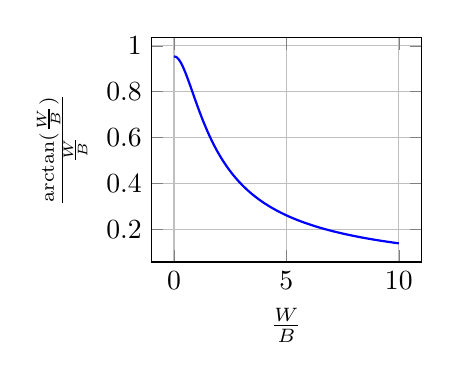
\begin{tikzpicture}
        \begin{axis}[
        domain=0.0001:10,
        xlabel=$\frac{W}{B}$,
        ylabel=$\frac{\arctan(\frac{W}{B})}{\frac{W}{B}}$,
        samples=100,
        smooth,
        scale=0.5,
        grid
        ]
        \addplot[blue,thick] {1/60*atan(x)/x};
        \end{axis}
      \end{tikzpicture}
  
  
    \end{figure}
    \end{columns}    
\end{frame}


\begin{frame}
  \frametitle{Questão 2}

  \begin{block}{Questão}
    Em um sistema de comunicação de radiodifusão, a 
    potência do transmissor é de 40 \si{\kilo\watt}, a atenuação do canal é de 80 dB e a
     potência de ruído é de $10^{-10}$ W/Hz.

     \begin{itemize}
      \item Encontre a SNR de pré-detecção.
      \item Encontre a SNR de saída se a modulação for DSB.
      \item Encontre a SNR de saída se a modulação for SSB.
      \item Encontre a SNR de saída se a modulação for AM convencional com um índice de modulação de 0,85 e possuir uma potência normalizada de mensagem de 0,2.
      \end{itemize}
  \end{block}

\end{frame}

\begin{frame}
  \frametitle{Solução}

  \begin{itemize}
    \item  Como a atenuação do canal é de 80 dB, então: 
    \begin{align*}
      P_R &= 10^{-8} \cdot P_T \\
        &= 10^{-8} \cdot 40 \cdot 10^3 \\
        & = 4 \cdot 10^{-4} \text{ Watts}
      \end{align*}
      Se o filtro limitador de ruído tem largura de banda B, então a potência de ruído pré-detecção é
      \begin{align*}
        P_n &= 2 \int_{f_c - B/2}^{f_c + B/2} \frac{N_0}{2}df = N_0B  \\
        & = 2 \times 10^{-10} B \text{Watts}.
      \end{align*}
    \item Portanto  : 
      \begin{equation*}
        SNR_{DSB,AM} = \frac{P_R}{P_n} = \frac{4\cdot 10^{-4}}{2 \cdot 10^{-10} \cdot 2 \cdot 10^4} = 100
        \end{equation*}
  \end{itemize}

\end{frame}

\begin{frame}
  \frametitle{Solução}
  \begin{itemize} 
    \item Para o caso SSB
  \begin{equation*}
    SNR_{SSB,AM} = \frac{P_R}{P_n} = \frac{4\cdot 10^{-4}}{2 \cdot 10^{-10} \cdot 10^4} = 200
    \end{equation*}
  
    \item $SNR_{DSB,o} = 2 SNR_{DSB,i} = 200 $
    \item $SNR_{SSB,o} = SNR_{SSB,i} = 200 $
    \item Sendo $\alpha = 0.8$ e $P_{M_n} = 0.2$ 
    \begin{equation}
      SNR_{AM,o} = \frac{\alpha^2 P_{M_n}}{1 + \alpha^2 P_{M_n}}SNR_{AM,i} = 0.1135 \cdot 2 \cdot 10^2
      \end{equation}
  \end{itemize}  

\end{frame}


\begin{frame}
  \frametitle{Questão 3}

  \begin{block}{Questão}
    Um canal de comunicação é caracterizado por uma atenuação de 90 dB e 
    por um ruído branco aditivo com densidade espectral de potência de 
    $0,5 x 10^{-14}$ W/Hz. A largura de banda da mensagem é de 1,5 MHz e 
    sua amplitude é uniformemente distribuída dentro do intervalo $[-1,1]$. 
    Se a SNR (razão sinal-ruído) necessária após a modulação é de 30 dB, 
    encontre a potência do transmissor em cada um dos casos.

    \begin{itemize}
      \item Modulação SSB.
      \item AM convencional com índice de modulação de 0,5 com potência normalizada 1/3.
      \item Modulação DSB-SC.
    \end{itemize}

  \end{block}

\end{frame}

\begin{frame}
  \frametitle{Solução}

  \begin{itemize}
    \item Primeiro passo é determinar a a SNR de banda-básica

    \begin{align*}
      \left(\frac{S}{N}\right) & = \frac{P_r}{N_0W} \\
      & = \frac{P_r}{2\cdot 0.5 \cdot 10^{-14} \cdot 1.5 \cdot 10^6} \\
      & = \frac{P_r10^8}{1.5}
    \end{align*}

    \item $P_r = 10^{-9}P_T$ 
    \item $\left(\frac{S}{N}\right) = \frac{P_r10^8}{1.5} = \frac{P_r}{15}$
  \end{itemize}

\end{frame}


\begin{frame}
  \frametitle{Solução}

  \begin{itemize}

    \item Portanto, a potência para o sistema SSB é

  \begin{align*}
    \left(\frac{S}{N}\right)_{SSB}  &= \left(\frac{S}{N}\right) = 10^3 \\
    P_T &= 15 \si{\kilo\watt}
  \end{align*}

  
    \item Para o caso AM-convencional tem-se que 
    \begin{align*}
      \left(\frac{S}{N}\right)_{AM-c} &= \frac{\alpha ^2 P_{M_n}}{1+\alpha ^2 P_{M_n}}\left(\frac{S}{N}\right) \\
      &=\frac{0.25 \cdot \frac{1}{3}}{1 + 0.25 \cdot \frac{1}{3}} \frac{P_T}{15} \\
      P_T& =195 \si{\kilo\watt}
    \end{align*}
  \end{itemize}
 
\end{frame}


\begin{frame}
  \frametitle{Solução}

  \begin{itemize}
    \item Similarmente ao caso SSB, tem-se que 
    \begin{align*}
      \left(\frac{S}{N}\right)_{SSB}  &= \left(\frac{S}{N}\right) = 10^3 \\
      P_T &= 15\si{\kilo\watt}
    \end{align*} 
  \end{itemize}  

\end{frame}




\section{Modulação FM}


\begin{frame}
  \frametitle{Questão 4}

  \begin{block}{Questão}
    O sinal de mensagem normalizado $m_n(t)$ tem uma largura de banda de 
    5 \si{\kilo \hertz} e uma potência de 0.1 \si{\watt}. O canal tem uma largura 
    de banda de 100 \si{\kilo \hertz} e uma atenuação em 80 dB. O ruído é branco com
    uma densidade espectral de potência $0,5 \times 10^{-12}$ \si{\watt \per \hertz} e a potência do transmissor é 
    10 \si{\kilo \watt}.  

    \begin{itemize}
      \item Se AM com índice de modulação $\alpha = 0.8$ , qual é  SNR de saída?
      \item Se FM é empregado, qual é a SNR mais alta possível?
    \end{itemize}

  \end{block}
  
\end{frame}


\begin{frame}
  \frametitle{Solução do item 1}
   A potência do sinal recebido pode ser encontrada como: 

  \begin{align*}
  10\log{\frac{P_T}{P_R}} &= 80\\
  P_R &= 10^{-8}P_T\\
  P_R &= 10^{-4} W 
  \end{align*}
  
  
  \begin{align*}
  \left(\frac{S}{N}\right)_o &= \frac{ \alpha^2 P_{Mn}}{1 + \alpha^2 P_{Mn}} \left(\frac{S}{N}\right)_b
  &= \frac{ \alpha^2 P_{Mn}}{1 + \alpha^2 P_{Mn}} \frac{P_R}{N_0W}
  \end{align*}
  

  Assim, com $P_R = 10^{-4}$, $P_{Mn} = 0.1$, $\alpha = 0.8$ e $$N_0W = 2 \times 0.5 \times 10^{-12} \times 5 \times 10^3 = 5 \times 10^{-9}$$
\vspace*{-1cm}

$$ \left(\frac{S}{N}\right)_o = 1204 \approx 30.806 dB $$

\end{frame}

\begin{frame}
  \frametitle{Solução do item 2}

  2. Usando a Regra de Carson, nós obtemos: 

\begin{align*}
B_c &= 2(\beta+1)W \\
100 \times 10^3 &= 2(\beta+1)5 \times 10^3 \\
\beta &= 9
\end{align*}

Verificamos agora se o limite impõe alguma restrição. 

\begin{align*}
\left(\frac{S}{N}\right)_{b,th} & = 20(\beta +1)\\
20000&= 20(\beta +1)\\
\beta &= 999
\end{align*} 

\end{frame}

\begin{frame}
  \frametitle{Solução do item 2}

  Como estamos limitados em largura de banda, escolhemos $\beta = 9$. *A relação sinal/ruído de saída é: 

\begin{align*}
\left(\frac{S}{N}\right)_{o} &= 3\beta^20.1\left(\frac{S}{N}\right)_{b}\\
&= 3 \times 9^2 \times0.1 \times \frac{10^5}{5}\\
&= 48600 \approx 56.866 db
\end{align*}

\end{frame}



\begin{frame}
  \frametitle{Questão 5}
\scriptsize
  \begin{block}{Questão}
    Um sinal de mensagem normalizado tem uma largura de banda de $W = 8 \si{\kilo \hertz}$
     e uma potência de $P_{Mn} = \frac{1}{2}$. É necessário transmitir este sinal 
     através de um canal com largura de banda disponível de 60 KHz e atenuação de 40 \si{\decibel}.
     O ruído do canal é aditivo e branco com uma densidade espectral de potência de 
     $\frac{N_0}{2} = 10^{-12}$ \si{\watt \per \hertz}. Um esquema de modulação de frequência, 
     sem filtragem de pré-ênfase/de-ênfase, foi proposto para esse fim.

     \begin{enumerate}
      \item Se for desejável ter um SNR de pelo menos 40 \si{\decibel} na saída do receptor, qual é a potência mínima necessária do transmissor e o índice de modulação correspondente?
      \item Se a SNR mínima exigida for aumentada para 60 \si{\decibel}, como sua resposta mudaria?
      \item Se na parte 2 pudermos empregar filtros de pré-ênfase/de-ênfase com uma constante de tempo de $\tau = 75 \si{\micro \second} $ , como a resposta da parte 2 mudaria?
    \end{enumerate}
    
  \end{block}

\end{frame}




\begin{frame}
  \frametitle{Solução do item 1}
  Primeiro, verificamos se o limite ou a largura de banda impõem um limite restritivo no índice de modulação. Pela regra de Carson temos:

\begin{align*}
B_c &= 2(\beta+1)W \\
60 \times 10^3 &= 2(\beta+1) 8 \times 10^3 \\
\beta &= 2.75
\end{align*}

Usando a relação $$\left(\frac{S}{N}\right)_o = 60 \beta^2(\beta+1)P_{Mn}$$


\end{frame}


\begin{frame}
  \frametitle{Solução do item 1}

  Com $ \left(\frac{S}{N}\right)_o = 10^4$ e $P_{Mn} = \frac{1}{2}$ nos encontramos: 

$$10^4 = 30 \beta^2(\beta+1)$$
$$\beta = 6.6158$$

Como estamos limitados em largura de banda, escolhemos $\beta = 2,75$. Então,

\begin{align*}
\left(\frac{S}{N}\right)_o &= 3\beta^2P_{Mn}\left(\frac{S}{N}\right)_b\\
\left(\frac{S}{N}\right)_b &= \frac{2 \times 10^4}{3 \times 2.75^2} \\
&= 881.542
\end{align*}


\end{frame}


\begin{frame}
  \frametitle{Solução do item 1}

  Assim, 

\begin{align*}
\left(\frac{S}{N}\right)_b &= \frac{P_R}{N_0W} = 881.542\\
P_R &= 881.542 \times 2 \times 10^{-12} \times 8 \times 10^3 \\
P_R &= 1.41 \times 10^{-5}
\end{align*}

omo a atenuação do canal é de 40 db, encontramos: 

$$P_T = 10^4P_R = 0.141 W$$


\end{frame}

\begin{frame}
  \frametitle{Solução do item 2}

  Se a SNR mínima exigida for aumentada para 60 db, então o $\beta$ da regra de Carson permanece o
mesmo, enquanto a partir da relação

$$\left(\frac{S}{N}\right)_o = 60 \beta^2(\beta+1)P_{Mn}= 10^6$$

Encontramos $\beta = 31,8531$. Como na parte 1), escolhemos $\beta = 2,75$ e, portanto,

\begin{align*}
\left(\frac{S}{N}\right)_b &= \frac{1}{3\beta^2P_{Mn}}\left(\frac{S}{N}\right)_o = 8.8154 \times 10^4
\end{align*}

\end{frame}


\begin{frame}
  \frametitle{Solução item 2}

  Assim, 

\begin{align*}
  P_R &= N_0W \times 8.8154 \times 10^4 \\
     &= 2 \times 10^{-12} \times 8 \times 10^3 \times 8.8154 \times 10^4 \\
     &= 0.0014
\end{align*}

e

$$P_T = 10^4 P_R = 14 W$$

\end{frame}


\begin{frame}
  \frametitle{Solução item 3}

  A resposta de frequência do filtro do receptor (de-ênfase) é dada por: 


$$H_d(f) = \frac{1}{1+j \frac{f}{f_0}}$$

Como $f_0 = \frac{1}{2 \pi \times 75 \times 10^{-6}} = 2100Hz$. Neste caso: 

\begin{align*}
\left(\frac{S}{N}\right){o,PD} =  \frac{\left(\frac{W}{f_0} \right)^3}{3 \left( \frac{W}{f_0} - arctan \frac{W}{f_0} \right)} \left(\frac{S}{N}\right){o} = 10^6 
\end{align*}



\end{frame}

\begin{frame}
  Assim temos 

$$
\left(\frac{S}{N}\right)_{o} = \frac{10^6}{\left( \frac{\left(\frac{8 \cdot 10^3}{2100}\right)^3}{3 \cdot\left(\frac{8 \cdot 10^3}{2100}-\arctan \left(\frac{8 \cdot 10^3}{2100}\right)\right)} \right)} = 1.3541 \times 10^5
$$


Com isso encontramos: 


$$ P_R = 9.55 \times 10^{-5}$$


e, portanto, 

$$P_T = 10^4P_R = 0.955W$$

\end{frame}

\section{Figura de Ruído}





\begin{frame}
  \frametitle{Questão 6}


  \begin{block}{Questão}
    Um amplificador possui largura de banda equivalente de 25 \si{\kilo\hertz} e ganho de 30 \si{\decibel}. A potência na saída é 
    de $10^8 k T_0$, em que $T_0$  define a temperatura ambiente. Determine a temperatura efetiva de ruído e a
    figura de ruído.
  \end{block}
  

\end{frame}








\begin{frame}
  \frametitle{Solução}

    Considere  que 

$$
P_{n_0} = GK B_{neq} (T + T_e)
$$
Substituindo os valores tem-se Questão
\begin{align*}
  P_{n_0} &= GK B_{neq} (T + T_e) \\
  10^8 k T_0&= 10^{3} \cdot k \cdot 25 \times 10^{3} (T_0 + T_e) \\
  T_e &= \frac{10^8 - 25 \times 10^{6}}{ 25 \times 10^{6}}T_0  \\
  &= \frac{75 \times 10^{6}}{ 25 \times 10^{6}}T_0  \\
  &= 3T_0  \\
\end{align*}
\end{frame}

\begin{frame}
  \frametitle{Solução}

  Portanto a figura de ruído é
$$
F = \left(1 + \frac{3T_0}{T_0}\right) = 4
$$ 

\end{frame}

\end{document}